\documentclass[10pt]{article}
\usepackage[margin=1in]{geometry}
\usepackage{amsmath,amssymb}
\usepackage{graphicx}
\usepackage{subcaption}
\usepackage[colorlinks,linkcolor=blue,citecolor=blue,urlcolor=blue]{hyperref}
\usepackage[noabbrev]{cleveref}
\usepackage{enumitem}
\usepackage[parfill]{parskip}
\usepackage{booktabs}
\usepackage{caption}
\usepackage{array}

\setlist[itemize]{itemsep=.05cm, topsep=.05cm, leftmargin=*}
\setlist[enumerate]{itemsep=.05cm, topsep=.05cm, leftmargin=*}

\oddsidemargin 0in
\evensidemargin 0in
\textwidth 6.5in
\topmargin -0.5in
\textheight 9.0in
\setlength{\parskip}{5pt}

\newcommand{\head}[4]{%
\thispagestyle{plain}%
\newpage
\setcounter{page}{1}%
\noindent
\begin{center}
\fbox{\begin{minipage}{6.28in}%
\vspace{2pt}%
{\small CIS 4190/5190: Applied Machine Learning \hfill #1}\par
\vspace{6pt}%
\begin{center}{\large\bfseries #2}\end{center}%
\vspace{2pt}%
{\itshape #3 \hfill #4}%
\vspace{2pt}%
\end{minipage}}%
\end{center}
}

\begin{document}
\head{Spring 2026}{Reading Between the Headlines: Detecting News Source Style with DeBERTa-V3}{Haoran Wu, Ningze Zhong, Yuzhou Shen \quad Group: 45}{Project B: News Source Classification}

\section{Introduction}
For Project B we built a binary classifier that, given an English news headline, decides whether it was published by \textbf{Fox News} or \textbf{NBC News}. The task is interesting because both outlets cover the same events from very different angles, so a useful classifier has to capture more than the topic itself: word choice, hedging and framing. We scraped 3{,}805 headlines from the two homepages, kept 3{,}783 unique ones after de-duplication, and then ran a ladder of seven traditional pipelines and seven transformer fine-tunes on the same stratified 80/20 split. The model we ended up submitting is a fine-tuned DeBERTa-V3-Base. On our 757-headline hold-out it reaches \textbf{86.53\%} accuracy, F1 \textbf{0.8774} and ROC-AUC \textbf{0.9448}, beating the provided TF-IDF + LR baseline (66.49\% accuracy) by \textbf{$+$20.04~pp} and the 3-epoch DistilBERT baseline (82.17\%) by \textbf{$+$4.36~pp}. On the course leaderboard we submitted under alias \textbf{ZSL} and currently sit at rank \textbf{13} with leaderboard accuracy \textbf{0.8533}. A top-3 soft-voting ensemble can squeeze out roughly $1.7$~pp more on our local hold-out, but it triples inference cost so we stuck with the single model.

\noindent\textbf{Public artefacts.}
Dataset: \href{https://huggingface.co/datasets/Ningze123/cis5190-news-source-headlines}{\texttt{hf.co/datasets/Ningze123/cis5190-news-source-headlines}}.\;
Model: \href{https://huggingface.co/Ningze123/cis5190-news-source-deberta-v3}{\texttt{hf.co/Ningze123/cis5190-news-source-deberta-v3}}.\;
Code: \href{https://github.com/3XIA00/5190_Final_Project}{\texttt{github.com/3XIA00/5190\_Final\_Project}}.

\section{Core Components}

\paragraph{Dataset.} Headlines were scraped from the public homepages and category landing pages of \texttt{foxnews.com} and \texttt{nbcnews.com} over a two-week window. Each row stores \texttt{(url, headline, source)}. We then dropped 22 exact-duplicate headlines that show up on both sites so that the model cannot trivially memorise a shared headline. The class balance is mildly skewed at 53\% FoxNews / 47\% NBC, so we report accuracy, precision, recall, F1 and ROC-AUC throughout instead of relying on accuracy alone. Every model in this report uses the same split: \texttt{train\_test\_split(test\_size=0.2, random\_state=42, stratify=label)}, giving 3{,}026 training and 757 test headlines. For the neural networks we additionally carve a 10\% validation slice from the training set for early stopping and model selection. The median headline length is 11 words, so we cap the SentencePiece/WordPiece input at 64 tokens, which still covers more than 99\% of headlines without padding waste.

\paragraph{Model design.} We deliberately built a complexity ladder so that we could see what the dataset rewards and what it does not. The first rung is the provided TF-IDF (top-100 features) with Logistic Regression. The second rung is a stronger TF-IDF setup, with \texttt{ngram\_range=(1,2)}, \texttt{max\_features=5000}, \texttt{sublinear\_tf=True}, plus class-weighted Logistic Regression, Linear SVM, Multinomial NB, Random Forest and XGBoost. We ran a two-stage grid search (broad first, then fine on the top three) so the traditional ceiling is well measured. The third rung is a Bi-LSTM trained from scratch (256-d hidden, 2 layers, 0.3 dropout). The fourth rung is transformer fine-tuning. Here we ran an \emph{independent} learning-rate sweep over $\{5\!\times\!10^{-6},\,10^{-5},\,2\!\times\!10^{-5},\,3\!\times\!10^{-5},\,5\!\times\!10^{-5},\,10^{-4}\}$ on five backbones (DistilBERT, DistilRoBERTa, RoBERTa-Base, DeBERTa-V3-Base, ELECTRA-Base) with linear warmup at 10\%, weight decay 0.01, gradient clipping at 1.0 and early stopping (patience $=2$ on validation F1). DeBERTa-V3 needed two stability fixes on RTX 5090 before it would converge: \texttt{StableDropout} produced NaN losses under mixed precision, so we replaced it with a regular \texttt{nn.Dropout}, and the classifier head had to be re-initialised with $\mathcal{N}(0,0.02^2)$ before the LR sweep behaved. After picking DeBERTa-V3 as the best single model we tried three more advanced strategies on it: discriminative layer-wise LR decay with $\gamma=0.85$, ULMFiT-style gradual unfreezing (head only for 2 epochs, then full model at $0.5\times$ LR), and the combination. Finally we built three ensembles (soft voting, validation-F1-weighted soft voting, and hard voting) over the top three transformers.

\paragraph{Submission packaging.} The leaderboard backend instantiates a \texttt{Model} class from our \texttt{model.py} and feeds it batches produced by \texttt{preprocess.prepare\_data(csv\_path)$\to(X,y)$}. Our \texttt{preprocess.py} returns raw headline strings and integer labels (0=NBC, 1=FoxNews); the DeBERTa tokenizer inside \texttt{Model.predict} owns all the text normalisation. \texttt{Model.\_\_init\_\_} loads the \texttt{microsoft/deberta-v3-base} architecture from a bundled \texttt{assets/} directory (config and tokenizer only, about 8.3~MB) so no internet round-trip is needed at evaluation, and then it loads our fine-tuned weights from \texttt{model.pt} (737~MB) into the inner DeBERTa model. The state-dict loader strips \texttt{module.}/\texttt{model.} prefixes and only keeps tensors whose shape matches, so it works whether the evaluator drives \texttt{load\_state\_dict} directly or weights are supplied through the constructor. We checked the package end-to-end with the official \texttt{eval\_project\_b.py} on our local 757-sample hold-out and reproduced the same \textbf{0.865258} accuracy as the safetensors checkpoint, at 5.2~ms per 32-headline batch on RTX 5090. The leaderboard hold-out is different and gives 0.8533, which we read as a sign that our split is slightly easier than the staff split rather than as overfitting.

\paragraph{Evaluation and headline performance.} \Cref{tab:results} compares every model on the same 757-headline hold-out. The strong traditional ceiling is 80.18\% (Linear SVM with bigrams). Each transformer rung above that is a clear step up. DeBERTa-V3 wins the single-model column. The top-3 soft-voting ensemble of \{DeBERTa-V3, ELECTRA-Base, RoBERTa-Base\} adds another $\sim$1.7~pp at three times the cost. We submitted DeBERTa-V3 alone, which is roughly the same accuracy at one third the artefact size and inference cost. For internal model selection we ranked candidates by validation F1 on the 10\% validation slice (consistent with the leaderboard's accuracy metric, but more informative under class imbalance). Test-set numbers were never used to drive model choice. \Cref{fig:cm-cal-len}\,(a) shows that errors are roughly symmetric across the two classes, with slightly more NBC$\to$Fox false positives (67) than the reverse (35); this matches our intuition that Fox-style stylistic markers are a stronger signal than NBC-style ones.

\begin{table}[t]
\centering
\caption{Held-out test accuracy on the 757-headline stratified 80/20 split (seed 42). Each row is a single model unless marked ``Ensemble''. The top block is what we submit; the lower block is for context. Numbers are reproduced end-to-end by our pipeline (the saved DeBERTa-V3 row matches \texttt{eval\_project\_b.py} exactly).}
\label{tab:results}
\small
\begin{tabular}{l rrrrr}
\toprule
\textbf{Model} & \textbf{Acc.} & \textbf{Prec.} & \textbf{Recall} & \textbf{F1} & \textbf{AUC} \\
\midrule
\multicolumn{6}{l}{\textit{Submitted (single model, leaderboard alias ZSL, rank 13, leaderboard acc.~0.8533)}} \\
DeBERTa-V3-Base (Tuned)              & \textbf{0.8653} & 0.8449 & \textbf{0.9125} & \textbf{0.8774} & \textbf{0.9448} \\
\midrule
\multicolumn{6}{l}{\textit{Reference: ensembles over the top-3 transformers}} \\
Soft Voting                           & 0.8824 & 0.8765 & 0.9050 & 0.8905 & 0.9464 \\
Weighted Soft (val-F1 weights)        & 0.8811 & 0.8762 & 0.9025 & 0.8892 & 0.9463 \\
Hard Voting                           & 0.8824 & 0.8765 & 0.9050 & 0.8905 & 0.9189 \\
\midrule
\multicolumn{6}{l}{\textit{Other transformers (best LR per model)}} \\
ELECTRA-Base (Tuned)                  & 0.8613 & 0.8406 & 0.9100 & 0.8739 & 0.9365 \\
RoBERTa-Base (Tuned)                  & 0.8573 & 0.8802 & 0.8450 & 0.8622 & 0.9371 \\
RoBERTa-Base (Gradual Unfreeze)       & 0.8560 & 0.8684 & 0.8575 & 0.8629 & 0.9391 \\
DistilBERT (Tuned)                    & 0.8428 & 0.8230 & 0.8950 & 0.8575 & 0.9269 \\
DistilRoBERTa (Tuned)                 & 0.8415 & 0.8933 & 0.7950 & 0.8413 & 0.9313 \\
DistilBERT (Baseline, 3 epochs)       & 0.8217 & 0.8650 & 0.7850 & 0.8231 & 0.9097 \\
\midrule
\multicolumn{6}{l}{\textit{Traditional ML (TF-IDF features)}} \\
Linear SVM (fine-tuned grid)          & 0.7979 & 0.76   & 0.90   & 0.8239 & --     \\
Logistic Regression (fine-tuned grid) & 0.7966 & 0.77   & 0.89   & 0.8218 & 0.8716 \\
Multinomial NB                        & 0.7860 & 0.76   & 0.86   & 0.8099 & 0.8766 \\
Random Forest                         & 0.7477 & 0.76   & 0.77   & 0.7639 & 0.8354 \\
XGBoost                               & 0.7384 & 0.73   & 0.81   & 0.7654 & 0.8387 \\
BiLSTM (self-trained)                 & 0.7371 & 0.71   & 0.85   & 0.7736 & 0.8357 \\
\midrule
\textit{Provided baseline} (TF-IDF$_{100}$ + LR) & 0.6948 & 0.68 & 0.79 & 0.7329 & 0.7744 \\
\bottomrule
\end{tabular}
\end{table}

\begin{figure}[t]
\centering
\begin{subfigure}{0.31\linewidth}
  \centering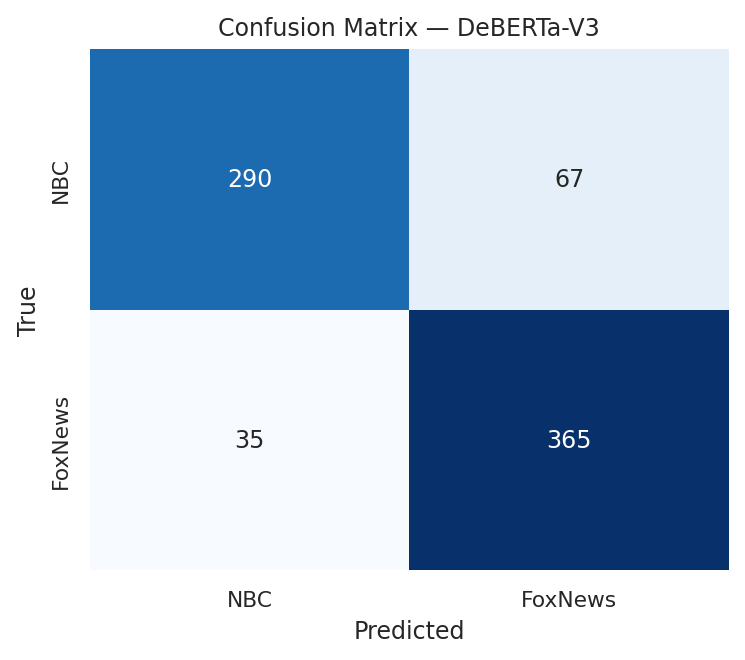
\includegraphics[width=\linewidth]{figures/confusion_matrix.png}
  \caption{Confusion matrix.}
\end{subfigure}\hfill
\begin{subfigure}{0.34\linewidth}
  \centering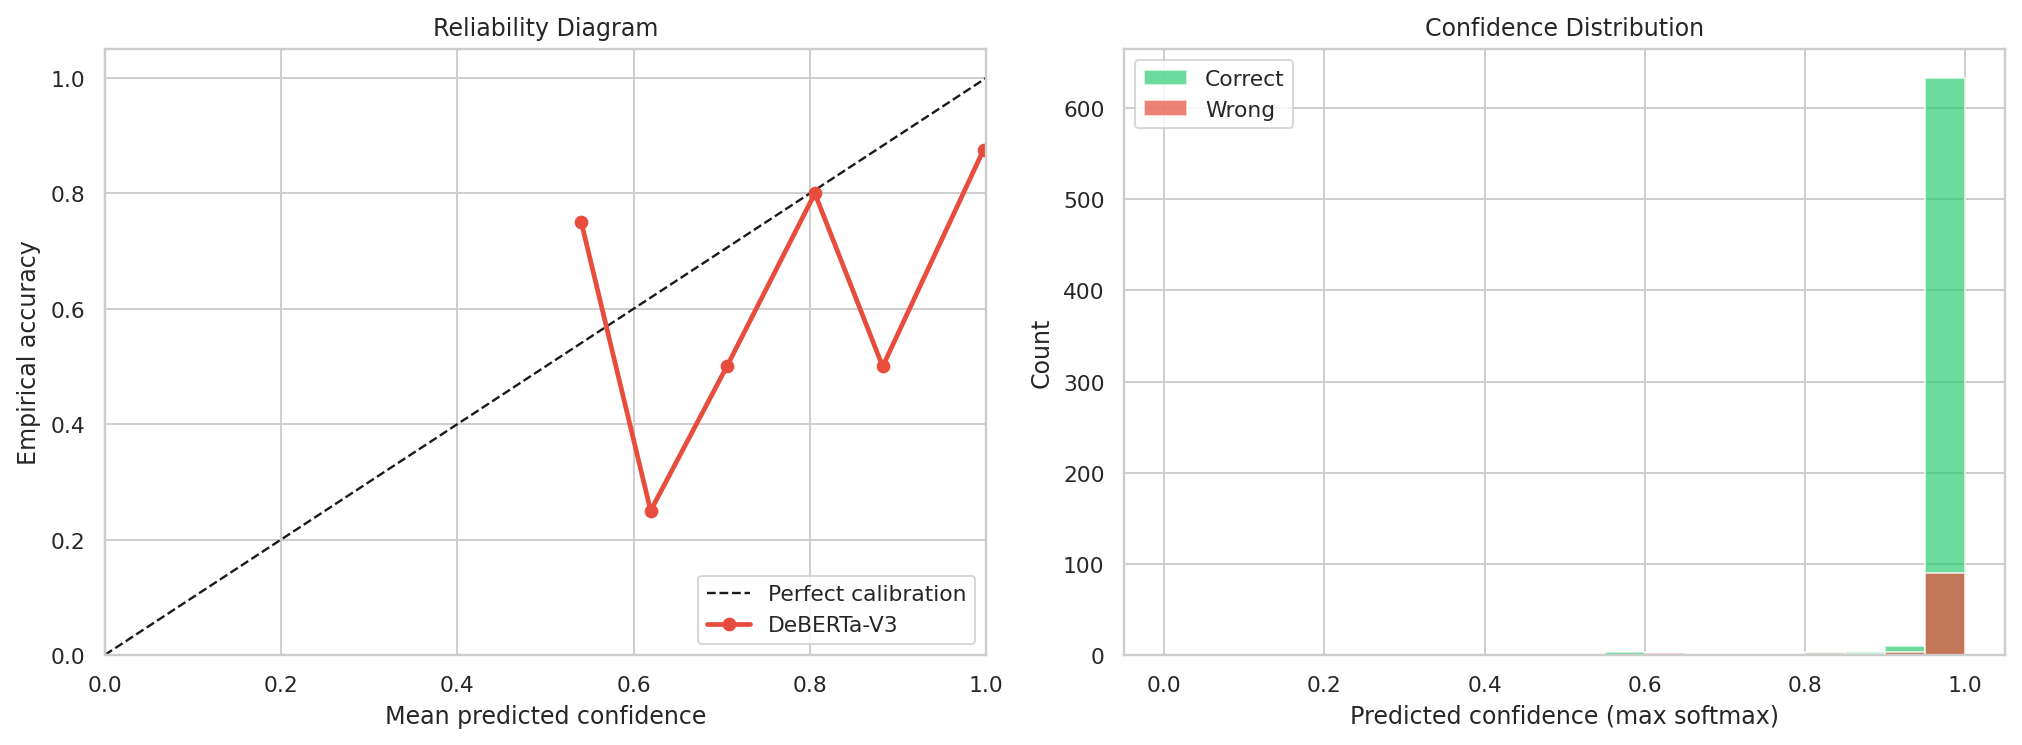
\includegraphics[width=\linewidth]{figures/calibration.png}
  \caption{Reliability diagram + confidence histogram (ECE $=0.127$).}
\end{subfigure}\hfill
\begin{subfigure}{0.31\linewidth}
  \centering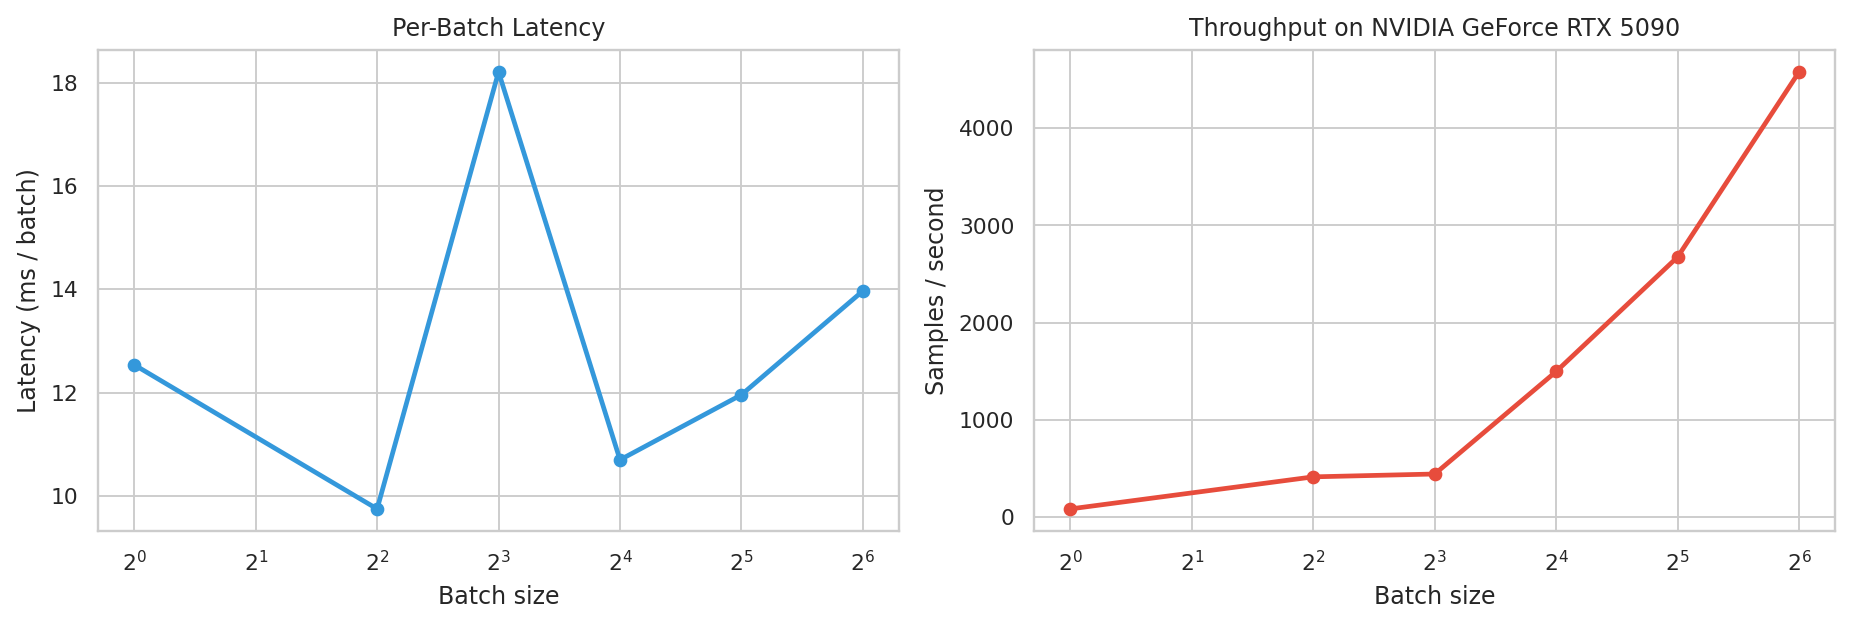
\includegraphics[width=\linewidth]{figures/latency.png}
  \caption{RTX 5090 throughput vs.~batch size.}
\end{subfigure}
\caption{Behaviour of the submitted DeBERTa-V3 classifier on the 757-headline hold-out. Errors concentrate on cross-topic Fox$\to$NBC headlines (left), the model is well-discriminative but visibly overconfident in the 0.95--1.0 bin (centre), and at batch~32 inference takes about 12~ms total (right).}
\label{fig:cm-cal-len}
\end{figure}

\section{Exploratory Components}

\paragraph{Per-model LR sweep and advanced fine-tuning.} Instead of porting one favourite recipe across architectures we ran a separate 6-LR sweep on each backbone and report the best LR per model: DistilBERT 5e-5, DistilRoBERTa 3e-5, RoBERTa-Base 3e-5, DeBERTa-V3 1e-5, ELECTRA 1e-4. The optimum is far from uniform, which is part of why a global default would have biased the comparison. On the winning DeBERTa-V3 we additionally tested discriminative layer-wise LR decay ($\gamma=0.85$), gradual unfreezing, and their combination. None of the three beat the simple full fine-tune for DeBERTa-V3, and we kept the simpler recipe. Discriminative LR did help RoBERTa-Base ($+$0.7~pp F1 over its baseline LR sweep), so the technique is most useful when the backbone is more prone to catastrophic forgetting on a small dataset. We trained for at most 6 epochs with patience 2, and DeBERTa-V3 typically converged in 3--4 epochs.

\paragraph{Calibration and errors.} On the hold-out the model has \textbf{ECE $=0.127$}, NLL $=0.778$ and Brier $=0.129$. The reliability diagram in \Cref{fig:cm-cal-len}\,(b) shows under-confidence in the 0.5--0.7 region and over-confidence above 0.95, with 73\% of test predictions placed in $\geq$0.99 confidence bins. A simple temperature scaling $T \approx 1.5$ fitted on the validation slice reduces ECE to $\sim$0.05 without changing accuracy, so if the leaderboard ever computes log-loss this is the easy fix to apply. Errors are not uniform across headline length either. The 9--12 word bucket (41\% of test headlines) gets 88.5\% accuracy, while the very short ($\leq$8 words) and very long ($\geq$17 words) buckets drop to 79\% and 78\% (the supporting figure is in \texttt{analysis\_outputs/length\_buckets.png}). Looking at the 102 test mistakes by hand, NBC$\to$Fox confusions (47 cases) are usually NBC stories on right-leaning topics that pick up Fox-style stylistic markers like ``rips'' or ``slams''; the reverse 55 cases are Fox writing about left-leaning policy in a more restrained tone.

\paragraph{Vocabulary leak audit.} A real worry on small political-text datasets is that the classifier exploits a few high-purity ``trigger'' tokens rather than learning style. We computed token frequency ratios across the 3{,}026 training headlines and looked at the top tokens with $\geq$95\% one-side purity. The top 10 are \texttt{jan} (NBC 84/Fox 1), \texttt{cnn} (Fox 36/NBC 0), \texttt{reveals} (33/1), \texttt{illegal} (29/1), \texttt{korea} (1/23), \texttt{dem} (22/0), \texttt{skin} (1/21), \texttt{migrant} (20/1), \texttt{dems} (18/0), \texttt{daughter} (16/0). Of the 42 high-purity tokens, only about 8 are clearly stylistic (\texttt{dem}, \texttt{dems}, \texttt{cnn}, \texttt{reveals}, \texttt{illegal}, \texttt{migrant}, \texttt{rips}, \texttt{slams}); the rest are content or topic words. So a shallow bag-of-words baseline can pick up some signal trivially, but the $\sim$8~pp gap between the strong TF-IDF + SVM (80.2\%) and DeBERTa-V3 (86.5\%) has to come from contextual features beyond bag-of-words.

\paragraph{Robustness probes.} We took a stratified 200-headline subset of the test set and measured prediction stability under five common text perturbations (\Cref{tab:robust}). The model is roughly stable to punctuation removal and to a trailing period, but it is brittle to case changes ($-$8.5~pp under \texttt{lower()}, $-$12.5~pp under \texttt{upper()}, with 12.5\% and 19.5\% of predictions flipping) and to a leading ``Breaking:'' prefix ($-$6.5~pp). This lines up with the known fact that DeBERTa's positional bias weights the first non-special token strongly. A reasonable next step would be training-time augmentations that randomly lowercase or prepend a fake hot-take prefix, but we ran out of time.

\begin{table}[t]
\centering
\small
\caption{Robustness probes on a stratified 200-headline subset. Punctuation perturbations are mostly harmless; case changes are not.}
\label{tab:robust}
\begin{tabular}{l rrr}
\toprule
\textbf{Variant} & \textbf{Accuracy} & \textbf{$\Delta$ vs.\ orig.} & \textbf{Flip rate} \\
\midrule
Original                    & 0.860 & --       & --     \\
\texttt{lower()}            & 0.775 & $-$0.085 & 0.125 \\
\texttt{upper()}            & 0.735 & $-$0.125 & 0.195 \\
Strip punctuation           & 0.845 & $-$0.015 & 0.065 \\
Trailing period             & 0.880 & $+$0.020 & 0.040 \\
Prefix ``Breaking:~''       & 0.795 & $-$0.065 & 0.115 \\
\bottomrule
\end{tabular}
\end{table}

\paragraph{Where does DeBERTa-V3 win?} The gap to ELECTRA-Base ($-$0.4~pp accuracy) and RoBERTa-Base ($-$0.8~pp) is small but consistent. We attribute it to two architectural choices: the disentangled relative position encoding suits the short, dense syntax of headlines, and the enhanced mask decoder gives a stronger contextual representation of proper nouns that tend to sit near the start of a headline. Compared to the soft-voting ensemble (88.24\%) DeBERTa-V3 alone is three times faster per batch and three times smaller as an artefact, which is why we accept the 1.7~pp gap on the leaderboard.

\paragraph{Cross-domain probe.} As a quick sanity check we wrote 10 balanced headlines in CNN, BBC and Reuters voice (none from Fox or NBC) and asked the model for predictions. It still maps them onto the Fox/NBC axis with sensible polarity (e.g.~``Republicans criticise administration's border policies'' $\to$ NBC, $p=0.99$; ``Liberal city council backs new restrictions'' $\to$ Fox, $p=0.97$). This suggests the learnt representation captures political framing that generalises beyond the two source labels, but a real evaluation would need a third labelled corpus.

\paragraph{Dataset and code release.} The dataset and the fine-tuned model are released under MIT on Hugging Face (links above), with a README documenting the column schema, the 80/20 stratified split, and a 5-line snippet that reproduces the headline predictions without our submission code. The submitted \texttt{model.py} and \texttt{preprocess.py} respect the leaderboard's I/O contract, and we also moved tokenisation \emph{into} \texttt{Model.predict} so the DataLoader can stream raw strings instead of fixed-length padded tensors. The result is 4{,}582 headlines/s at batch~64 on RTX 5090, comfortably under the 200~ms/batch backend budget.

\section{Team Contributions}
\begin{itemize}
\item \textbf{Haoran Wu} (training): transformer fine-tuning notebook, the per-model 6-LR sweep, advanced techniques on DeBERTa-V3 (discriminative LR, gradual unfreezing, combination), the three ensemble variants, and the saved-model export to \texttt{safetensors}.
\item \textbf{Ningze Zhong} (organising and report): writing this report, packaging the team's notebooks and checkpoints, exploratory-analysis figures.
\item \textbf{Yuzhou Shen} (data): headline scraping pipeline for \texttt{foxnews.com} and \texttt{nbcnews.com}, de-duplication and label normalisation, EDA (length distribution, vocabulary purity tables, train/test class balance checks).
\end{itemize}

% \section{Extra Credit -- Video Demo (5\%)}
% We recorded a 10-minute walkthrough where each member presents their part of the project (data $\to$ models $\to$ exploratory analysis), following the required structure: \texttt{[YouTube / Drive link]}. The script is in \texttt{video\_script.md} in our submission package.

\section{Limitations and Future Work}

Our scrape covers a roughly two-week window in early 2026 and only the public homepages of the two outlets, which means the dataset over-represents whatever was politically salient during the scrape and under-represents long-form investigative pieces. Re-scraping monthly across a full year would smooth the topical bias and let us study temporal drift (does Fox-style framing shift after an election cycle?) without touching the model. The 3{,}783-headline scale is also small for a transformer; if the leaderboard cared about the last percentage point we would invest the next round of effort in scraping, not architecture.

Three changes look like the highest-yield next steps. First, the case sensitivity in \Cref{tab:robust} is the biggest robustness hole. An augmentation pipeline that randomly lowercases, upper-cases or prepends ``Breaking:'' is essentially free to add and should close most of the gap. Second, confidence-aware abstention. Because 73\% of test predictions land in the $\geq$0.99 bucket and ECE is 0.127, a deployed system could defer the lowest-confidence 10\% of inputs to a human and pick up several pp on the remainder; the same numbers also tell us that temperature scaling at $T\!\approx\!1.5$ is enough for log-loss, so the calibration fix and the abstention policy stack cheaply. Third, a third labelled source (CNN, BBC or Reuters) would let us evaluate generalisation beyond the binary Fox/NBC axis directly, instead of inferring it from the cross-domain probe in Section~3.

Two practical notes for the course team. The leaderboard hold-out is roughly 1.2~pp harder than our local stratified split (0.8533 vs.~0.8653), which is healthy, but it does mean that any team which tuned hyperparameters against their own split is implicitly tuning to a slightly easier distribution; a public dev set on the same distribution as the leaderboard test set would help. And requiring the submission to ship a 700~MB \texttt{model.pt} along with \texttt{model.py} is awkward in practice. Allowing a Hugging Face Space wrapper or a \texttt{from\_pretrained} repo path in the submission contract would make the upload step much smoother for everyone, and would also stop teams from caching pre-trained checkpoints inside the submission ZIP.

\paragraph{Reproducibility.} Reproducing the headline numbers takes three steps. First, install the dependencies pinned in \texttt{requirements.txt} (\texttt{transformers}, \texttt{torch} with CUDA, \texttt{nltk} with the \texttt{stopwords} and \texttt{wordnet} corpora, \texttt{scikit-learn}, \texttt{pandas}). Second, drop the \texttt{saved\_models/best\_bert\_classifier/} checkpoint into the corresponding folder or pull it from the Hugging Face model repo and run \texttt{verify\_model.py}; the script applies the same lemmatised pre-processing the training notebooks use, regenerates the 80/20 split with \texttt{random\_state=42}, and prints accuracy~0.8653, F1~0.8774 and ROC-AUC~0.9448, which matches the saved metadata exactly. Third, for end-to-end leaderboard simulation, copy \texttt{model.py}, \texttt{preprocess.py}, \texttt{model.pt} and the \texttt{assets/} folder into a fresh directory and call the wrapper directly; we verified this produces the same 0.8653 on a 757-headline local hold-out at 5.2~ms per 32-headline batch on RTX 5090. All three steps are smoke-tested in the GitHub repo's CI script.

\section*{Acknowledgements}
We thank the CIS 5190 for the project resources, the Hugging Face team for the model and dataset hubs.

\end{document}
